\section{Conclusion}

\begin{frame}{Conclusion: Spectral GNNs}
    \begin{itemize}
        \item \destaq{Spectral GNNs:}
        \begin{itemize}
            \item Best suited for capturing global, structural patterns and long-range dependencies in fixed networks.
            \item Works well in applications where the relationships span across the graph, making full use of spectral decomposition.
            \item \textbf{Example:} In biological networks like protein interactions, where complex, long-range dependencies are critical, spectral GNNs can effectively capture these intricate patterns.
        \end{itemize}
    \end{itemize}
\end{frame}

\begin{frame}{Conclusion: Graph Attention Networks (GAT)}
    \begin{itemize}
        \item \destaq{Graph Attention Networks (GAT):}
        \begin{itemize}
            \item Highly effective for tasks with localized, node-to-neighbor interactions, especially when directionality and edge features are important.
            $$ \alpha_{ij} = \sigma(\phi_1( \mathbf{a}^T [ W h_i || W h_j || W_2 e_{ij} ])) \; \text{where } e_{ij} \; \text{are edge features}$$
            \item The attention mechanism in GAT allows for selective focus on relevant neighboring nodes, making it ideal for relational data.
            \item \textbf{Example:} In airport flight networks, where each flight has unique characteristics (e.g., weather, fuel) and directionality matters, GAT can leverage these edge features for enhanced predictive accuracy.
        \end{itemize}
    \end{itemize}
\end{frame}

\begin{frame}{Airport Network: GAT application}

    \begin{figure}[ht]
    \centering
    \begin{tikzpicture}[
        ->, % directed edges
        >=stealth, % arrow tip
        node distance=3cm, % distance between nodes
        airport/.style={circle, draw, minimum size=2cm, font=\Large}, % style for airports
        flight/.style={font=\small} % style for flights
    ]

    % Nodes (Airports)
    \node[airport] (A) {SP \\ \faPlaneDeparture}; % São Paulo with departure icon
    \node[airport] (B) [right of=A] {RJ \\ \faPlaneDeparture}; % Rio de Janeiro with departure icon
    \node[airport] (C) [below of=A] {MG \\ \faPlaneDeparture}; % Minas Gerais with departure icon

    % Edges (Flights)
    \draw[->] (A) to node[flight, above] {\tikz[baseline]{\node[rotate=0]{\faPlane};}} (B); % Flight from SP to RJ, plane icon aligned (0 degrees)
    \draw[->] (B) to node[flight, right] {\tikz[baseline]{\node[rotate=220]{\faPlane};}} (C); % Flight from RJ to MG, plane icon rotated 270 degrees
    \draw[->] (C) to node[flight, left] {\tikz[baseline]{\node[rotate=96]{\faPlane};}} (A); % Flight from MG to SP, plane icon rotated 135 degrees

    \end{tikzpicture}
    \caption{Airports and Directed Flights}
    \label{fig:flight_network_graph}
\end{figure}

\end{frame}

\begin{frame}{Choosing the Right Model}
    \begin{itemize}
        \item \textbf{Spectral GNNs:} Suitable for applications requiring a deep understanding of global structures and where long-range relationships play a crucial role.
        \item \textbf{GAT:} Ideal for applications with localized interactions and rich edge features, especially in directed, dynamic networks.
    \end{itemize}
    \begin{block}{Key Insight}
        The decision between using Spectral GNNs or GAT largely depends on the graph's structure and the task's requirements. Spectral GNNs capture global connectivity patterns, while GAT's attention mechanism makes it better suited for applications where direction and edge-specific information are essential.
    \end{block}
\end{frame}